\section{GIF}

\subsection{Pourquoi le GIF?}
Le format GIF permet de stocker plusieurs images dans un fichier. 
Ceci permet de créer des diaporamas, voire des animations si les images sont affichées à un rythme suffisamment soutenu. 
Chaque image d'une animation peut avoir sa propre palette.
Le GIF est un format très utilisé, particulièrement sur les réseaux sociaux. 
Ce projet peut donc intéressé pas mal de gens.\\
La structure du format GIF est connue et disponible en ligne. En voici un schéma :

\vspace{1.5cm}

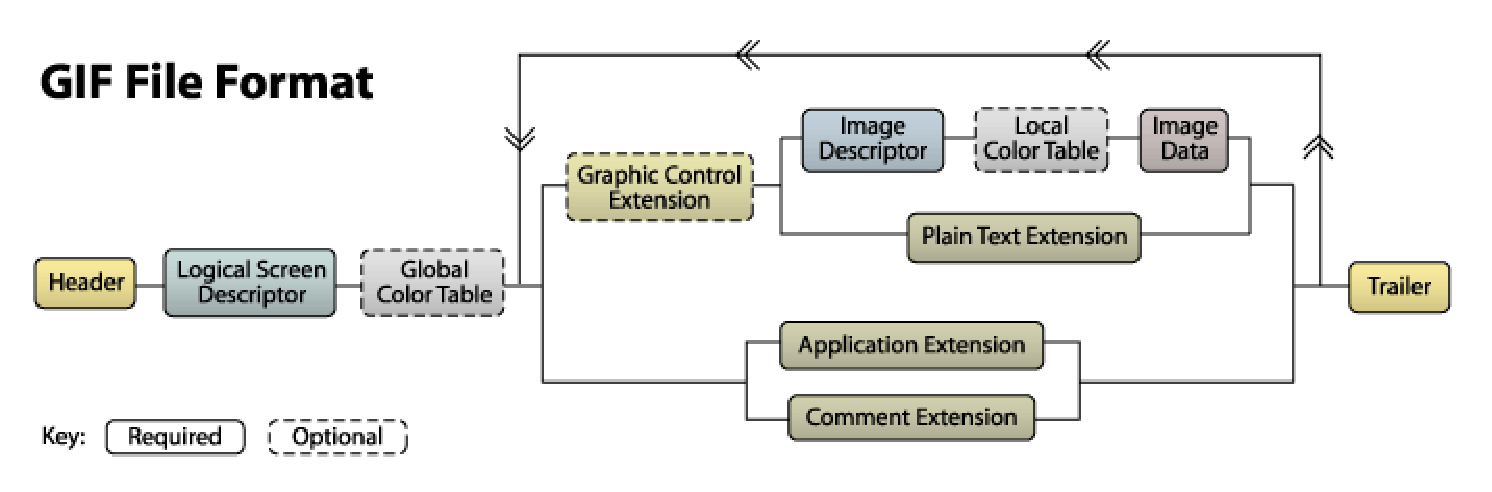
\includegraphics[width=15cm]{gif_structure.eps}


\newpage
\subsection{Application du LSB}
Nous avons choisi de cacher des informations dans les pixels qui se trouvent dans les Local Color Table car il s'agit d'une
suite de pixels qui ne sont soumis à aucune compression contrairement au segment d'image data.
Cette section facultative peut revenir devant chaque bloc image data. Si cette section n'existe pas, nous la rajoutons en copiant
alors la global color table à l'emplacement où elle aurait été c'est-à-dire juste devant le bloc image data.
On aura autant de color table qu'il n'y a de blocs image data.

Il est possible de calculer la taille maximale du message cachée à l'avance : 
en comptant le nombre de bloc image data et en le multipliant par le nombre de byte dans la Global Color Table.

\vspace{1.5cm}

\includemedia[width=0.45\linewidth,height=0.45\linewidth,activate=pageopen,
passcontext,
transparent,
addresource=dog_src.mp4,
flashvars={source=dog_src.mp4}
]{\includegraphics[width=0.45\linewidth]{dog_src.png}}{VPlayer.swf}